\documentclass[11pt, compress]{beamer}
\usepackage{amsmath}
\usetheme{Boadilla}
\usefonttheme[onlymath]{serif}
%get rid of navigation:
\setbeamertemplate{navigation symbols}{}


 %%%% Start PreTeXt generated preamble: %%%%% 

\newcommand{\tabularfont}{}
\usepackage[xparse, raster]{tcolorbox}
\tcbset{colback=white, colframe=white}
\NewTColorBox{image}{mmm}{boxrule=0.25pt, colframe=gray, left skip=#1\linewidth,width=#2\linewidth}
\RenewTColorBox{definition}{m}{colback=teal!30!white, colbacktitle=teal!30!white, coltitle=black, colframe=gray, boxrule=0.5pt, sharp corners=downhill, titlerule = 0.25pt, title={#1}}
\RenewTColorBox{theorem}{m}{colback=pink!30!white, colbacktitle=pink!30!white, coltitle=black, colframe=gray, boxrule=0.5pt, sharp corners=downhill, titlerule = 0.25pt, title={#1}}
\RenewTColorBox{proof}{}{boxrule=0.25pt, colframe=gray, colback=white, before upper={Proof:}, after upper={\qed}}
%% tcolorbox styles for sidebyside layout
\tcbset{ bwminimalstyle/.style={size=minimal, boxrule=-0.3pt, frame empty,
colback=white, colbacktitle=white, coltitle=black, opacityfill=0.0} }
\tcbset{ sbsstyle/.style={raster before skip=2.0ex, raster equal height=rows, raster force size=false} }
\tcbset{ sbspanelstyle/.style={bwminimalstyle} }
%% Enviroments for side-by-side and components
%% Necessary to use \NewTColorBox for boxes of the panels
%% "newfloat" environment to squash page-breaks within a single sidebyside
%% "xparse" environment for entire sidebyside
\NewDocumentEnvironment{sidebyside}{mmmm}
  {\begin{tcbraster}
    [sbsstyle,raster columns=#1,
    raster left skip=#2\linewidth,raster right skip=#3\linewidth,raster column skip=#4\linewidth]}
  {\end{tcbraster}}
%% "tcolorbox" environment for a panel of sidebyside
\NewTColorBox{sbspanel}{mO{top}}{sbspanelstyle,width=#1\linewidth,valign=#2}
\newcommand{\terminology}[1]{\textbf{#1}}\newcommand{\lt}{<}
\newcommand{\gt}{>}
\newcommand{\amp}{&}


\renewcommand{\d}{\displaystyle}
\newcommand{\N}{\mathbb N}
\newcommand{\B}{\mathbf B}
\newcommand{\Z}{\mathbb Z}
\newcommand{\Q}{\mathbb Q}
\newcommand{\R}{\mathbb R}
\newcommand{\C}{\mathbb C}
\newcommand{\U}{\mathcal U}
\newcommand{\pow}{\mathcal P}
\newcommand{\inv}{^{-1}}
\newcommand{\st}{:}
\renewcommand{\iff}{\leftrightarrow}
\newcommand{\Iff}{\Leftrightarrow}
\newcommand{\imp}{\rightarrow}
\newcommand{\Imp}{\Rightarrow}
\newcommand{\isom}{\cong}

\renewcommand{\bar}{\overline}
\newcommand{\card}[1]{\left| #1 \right|}
\newcommand{\twoline}[2]{\begin{pmatrix}#1 \\ #2 \end{pmatrix}}

\newcommand{\vtx}[2]{node[fill,circle,inner sep=0pt, minimum size=4pt,label=#1:#2]{}}
\newcommand{\va}[1]{\vtx{above}{#1}}
\newcommand{\vb}[1]{\vtx{below}{#1}}
\newcommand{\vr}[1]{\vtx{right}{#1}}
\newcommand{\vl}[1]{\vtx{left}{#1}}
\renewcommand{\v}{\vtx{above}{}}

%% Graphics Preamble Entries
\usepackage{tikz, pgfplots}

\usetikzlibrary{positioning,matrix,arrows}

\usetikzlibrary{shapes,decorations,shadows,fadings,patterns}
\usetikzlibrary{decorations.markings}

\usepackage{skak} %for chessboards etc.

\def\circleA{(-.5,0) circle (1)}
\def\circleAlabel{(-1.5,.6) node[above]{$A$}}
\def\circleB{(.5,0) circle (1)}
\def\circleBlabel{(1.5,.6) node[above]{$B$}}
\def\circleC{(0,-1) circle (1)}
\def\circleClabel{(.5,-2) node[right]{$C$}}
\def\twosetbox{(-2,-1.4) rectangle (2,1.4)}
\def\threesetbox{(-2.5,-2.4) rectangle (2.5,1.4)}
\newcommand{\hexbox}[3]{
  \def\x{-cos{30}*\r*#1+cos{30}*#2*\r*2}
  \def\y{-\r*#1-sin{30}*\r*#1}
  \draw (\x,\y) +(90:\r) -- +(30:\r) -- +(-30:\r) -- +(-90:\r) -- +(-150:\r) -- +(150:\r) -- cycle;
  \draw (\x,\y) node{#3};
}

\tikzset{->-/.style={decoration={
  markings,
  mark=at position .5 with {\arrow{>}}},postaction={decorate}}}

  \newcommand{\onedot}{
    +(.5,.5) \v
  }
  \newcommand{\twodots}{
    +(.25,.25) \v +(.75,.75) \v
  }
  \newcommand{\threedots}{
  +(.25,.25) \v +(.5, .5) \v +(.75,.75) \v
  }
  \newcommand{\fourdots}{
    +(.25,.25) \v +(.25,.75) \v +(.75,.25) \v +(.75,.75) \v
  }
  \newcommand{\fivedots}{
    +(.5,.5) \v +(.25,.25) \v +(.25,.75) \v +(.75,.25) \v +(.75,.75) \v
  }
  \newcommand{\sixdots}{
    +(.25,.5) \v +(.75,.5) \v +(.25,.25) \v +(.25,.75) \v +(.75,.25) \v +(.75,.75) \v
  }
  \newcommand{\dominoborder}{
    \draw[thick, rounded corners] (0,0) rectangle (1,2);
    \draw[thin] (0,1) -- (1,1);
  }


%%%% End of PreTeXt generated preamble %%%%% 

\title{What is Discrete Mathematics?}
\subtitle{}
\author{}
\date{}

\begin{document}
\begin{frame}
\maketitle 
\end{frame}
 
\begin{frame}
\frametitle{Overview}
\tableofcontents 
\end{frame}
 

\section{}
\begin{frame}
\frametitle{What is Discrete Mathematics?}
 \terminology{dis\textperiodcentered{} crete \slash{} dis'krët.}
 \emph{Adjective}: Individually separate and distinct.
 \emph{Synonyms}: separate - detached - distinct - abstract.
 
\pause \vfill 

Whatever your conception of what mathematics is, try applying the concept of ``discrete'' to it, as defined above. Some math fundamentally deals with \emph{stuff} that is individually separate and distinct.
\end{frame}
 
\begin{frame}
\frametitle{Example problem 1}
 \begin{example}[]The most popular mathematician in the world is throwing a party for all of his friends. As a way to kick things off, they decide that everyone should shake hands. Assuming all 10 people at the party each shake hands with every other person (but not themselves, obviously) exactly once, how many handshakes take place?
\end{example}
\end{frame}
 
\begin{frame}
\frametitle{Example problem 2}
 \begin{example}[]At the warm-up event for Oscar's All Star Hot Dog Eating Contest, Al ate one hot dog. Bob then showed him up by eating three hot dogs. Not to be outdone, Carl ate five. This continued with each contestant eating two more hot dogs than the previous contestant. How many hot dogs did Zeno (the 26th and final contestant) eat? How many hot dogs were eaten all together?
\end{example}
\end{frame}
 
\begin{frame}
\frametitle{Example problem 3}
 \begin{example}[]After excavating for weeks, you finally arrive at the burial chamber. The room is empty except for two large chests. On each is carved a message (strangely in English):
\begin{sidebyside}{1}{0.1}{0.1}{0}%
\begin{sbspanel}{0.8}%
\resizebox{\linewidth}{!}{%
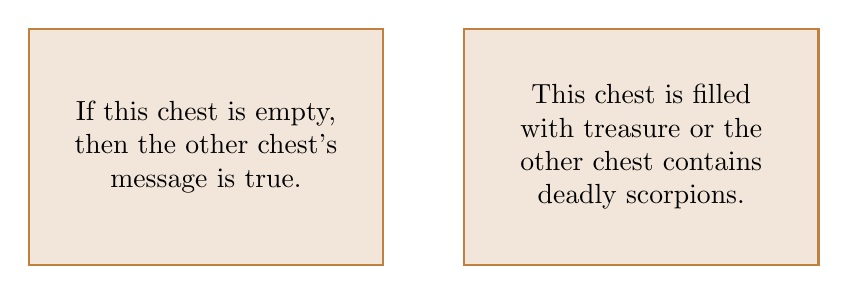
\begin{tikzpicture} \node[shape=rectangle, draw=brown, thick, fill=brown!20!white, inner sep=5mm, minimum height=3cm, minimum width=3.5cm, text width=3.5cm, align=center] (a) { If this chest is empty, then the other chest's message is true.}; \node[shape=rectangle, draw=brown, thick, fill=brown!20!white, inner sep=5mm, minimum height=3cm, minimum width=3.5cm, text width=3.5cm, align=center, right=of a] {
                      This chest is filled with treasure or the other chest contains deadly scorpions.
                      };
              \end{tikzpicture}
}%
\end{sbspanel}%
\end{sidebyside}%
You know exactly one of these messages is true. What should you do?
\end{example}
\end{frame}
 
\begin{frame}
\frametitle{Example problem 4}
 \begin{example}[]Back in the days of yore, five small towns decided they wanted to build roads directly connecting each pair of towns. While the towns had plenty of money to build roads as long and as winding as they wished, it was very important that the roads not intersect with each other (as stop signs had not yet been invented). Also, tunnels and bridges were not allowed. Is it possible for each of these towns to build a road to each of the four other towns without creating any intersections?
\end{example}
\end{frame}
 
\begin{frame}
\frametitle{Summary}
 Each of the problems above illustrate one of the main topics we will discuss in this course.
\pause 

\begin{itemize}[<+->]
\item{} Discrete mathematics deals with counting \emph{how many} ways something can happen.  We will learn how to count in chapter 1.


\item{} Discrete mathematics deals with manipulating sequences of numbers.  We will investigate this in chapter 2.


\item{} Discrete mathematics deals with logic, which also helps us understand how to prove our solutions to problems are correct.  We will do both of these in chapter 3.


\item{} Discrete mathematics deals with the ways things can be \emph{related}.  These relationships can be modeled using \emph{graphs}, which we will study in chapter 4.

\end{itemize}

 
\pause \vfill 

But first, we will review some basic mathematical tools that will help us study these questions.
\end{frame}
 

\end{document}
